\tikzstyle{vertex}=[draw,thick,circle,minimum size=2mm,inner sep=0pt]
\tikzstyle{edge} = [draw,thick,-]
\tikzstyle{weight} = [font=\small]

\newcommand{\cgscale}{0.6}
\newcommand{\cgpadv}{1mm}
\newcommand{\cgpadh}{1cm}

\newcommand{\An}{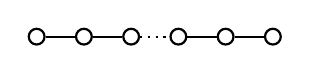
\begin{tikzpicture}[scale=\cgscale, auto, swap]
    % First we draw the vertices
    \foreach \pos/\name in {{(0,0)/a}, {(1,0)/b}, {(2,0)/c}, {(3,0)/d}, {(4,0)/e}, {(5,0)/f}}
        \node[vertex] (\name) at \pos {}; %{$\name$};
    % Connect vertices with edges and draw weights
    \foreach \source/ \dest /\weight in {a/b/,b/c/,d/e/,e/f/}
        \path[edge] (\source) -- node[weight] {$\weight$} (\dest);

    \path[edge, dotted] (c) -- node[weight] {} (d);
\end{tikzpicture}}

\newcommand{\Bn}{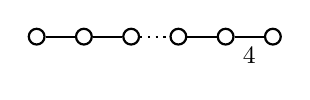
\begin{tikzpicture}[scale=\cgscale, auto, swap]
    % First we draw the vertices
    \foreach \pos/\name in {{(0,0)/a}, {(1,0)/b}, {(2,0)/c}, {(3,0)/d}, {(4,0)/e}, {(5,0)/f}}
        \node[vertex] (\name) at \pos {}; %{$\name$};
    % Connect vertices with edges and draw weights
    \foreach \source/ \dest /\weight in {a/b/,b/c/,d/e/,e/f/4}
        \path[edge] (\source) -- node[weight] {$\weight$} (\dest);

    \path[edge, dotted] (c) -- node[weight] {} (d);
\end{tikzpicture}}

\newcommand{\Dn}{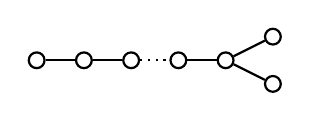
\begin{tikzpicture}[scale=\cgscale, auto, swap]
    % First we draw the vertices
    \foreach \pos/\name in {{(0,0)/a}, {(1,0)/b}, {(2,0)/c}, {(3,0)/d}, {(4,0)/e}, {(5,-0.5)/f}, {(5,0.5)/g}}
        \node[vertex] (\name) at \pos {}; %{$\name$};
    % Connect vertices with edges and draw weights
    \foreach \source/ \dest /\weight in {a/b/,b/c/,d/e/,e/f/,e/g/}
        \path[edge] (\source) -- node[weight] {$\weight$} (\dest);

    \path[edge, dotted] (c) -- node[weight] {} (d);
\end{tikzpicture}}

\newcommand{\Esix}{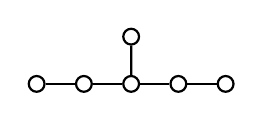
\begin{tikzpicture}[scale=\cgscale, auto, swap]
    % First we draw the vertices
    \foreach \pos/\name in {{(0,0)/a}, {(1,0)/b}, {(2,0)/c}, {(3,0)/d}, {(4,0)/e}, {(2,1)/f}}
        \node[vertex] (\name) at \pos {}; %{$\name$};
    % Connect vertices with edges and draw weights
    \foreach \source/ \dest /\weight in {a/b/,b/c/,c/d/,d/e/,c/f/}
        \path[edge] (\source) -- node[weight] {$\weight$} (\dest);
\end{tikzpicture}}

\newcommand{\Eseven}{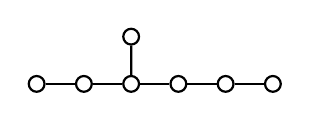
\begin{tikzpicture}[scale=\cgscale, auto, swap]
    % First we draw the vertices
    \foreach \pos/\name in {{(0,0)/a}, {(1,0)/b}, {(2,0)/c}, {(3,0)/d}, {(4,0)/e}, {(5,0)/f}, {(2,1)/g}}
        \node[vertex] (\name) at \pos {}; %{$\name$};
    % Connect vertices with edges and draw weights
    \foreach \source/ \dest /\weight in {a/b/,b/c/,c/d/,d/e/,e/f/,c/g/}
        \path[edge] (\source) -- node[weight] {$\weight$} (\dest);
\end{tikzpicture}}

\newcommand{\Eeight}{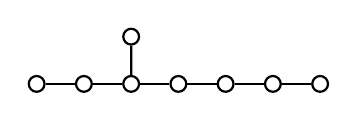
\begin{tikzpicture}[scale=\cgscale, auto, swap]
    % First we draw the vertices
    \foreach \pos/\name in {{(0,0)/a}, {(1,0)/b}, {(2,0)/c}, {(3,0)/d}, {(4,0)/e}, {(5,0)/f}, {(6,0)/g}, {(2,1)/h}}
        \node[vertex] (\name) at \pos {}; %{$\name$};
    % Connect vertices with edges and draw weights
    \foreach \source/ \dest /\weight in {a/b/,b/c/,c/d/,d/e/,e/f/,f/g/,c/h/}
        \path[edge] (\source) -- node[weight] {$\weight$} (\dest);
\end{tikzpicture}}

\newcommand{\Ffour}{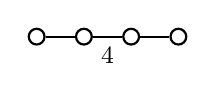
\begin{tikzpicture}[scale=\cgscale, auto, swap]
    % First we draw the vertices
    \foreach \pos/\name in {{(0,0)/a}, {(1,0)/b}, {(2,0)/c}, {(3,0)/d}}
        \node[vertex] (\name) at \pos {}; %{$\name$};
    % Connect vertices with edges and draw weights
    \foreach \source/ \dest /\weight in {a/b/,b/c/4,c/d/}
        \path[edge] (\source) -- node[weight] {$\weight$} (\dest);
\end{tikzpicture}}

\newcommand{\Hthree}{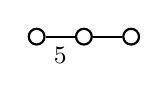
\begin{tikzpicture}[scale=\cgscale, auto, swap]
    % First we draw the vertices
    \foreach \pos/\name in {{(0,0)/a}, {(1,0)/b}, {(2,0)/c}}
        \node[vertex] (\name) at \pos {}; %{$\name$};
    % Connect vertices with edges and draw weights
    \foreach \source/ \dest /\weight in {a/b/5,b/c/}
        \path[edge] (\source) -- node[weight] {$\weight$} (\dest);
\end{tikzpicture}}

\newcommand{\Hfour}{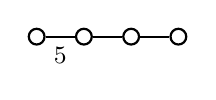
\begin{tikzpicture}[scale=\cgscale, auto, swap]
    % First we draw the vertices
    \foreach \pos/\name in {{(0,0)/a}, {(1,0)/b}, {(2,0)/c}, {(3,0)/d}}
        \node[vertex] (\name) at \pos {}; %{$\name$};
    % Connect vertices with edges and draw weights
    \foreach \source/ \dest /\weight in {a/b/5,b/c/,c/d/}
        \path[edge] (\source) -- node[weight] {$\weight$} (\dest);
\end{tikzpicture}}

\newcommand{\Itwom}{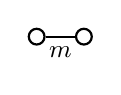
\begin{tikzpicture}[scale=\cgscale, auto, swap]
    % First we draw the vertices
    \foreach \pos/\name in {{(0,0)/a}, {(1,0)/b}}
        \node[vertex] (\name) at \pos {}; %{$\name$};
    % Connect vertices with edges and draw weights
    \foreach \source/ \dest /\weight in {a/b/m}
        \path[edge] (\source) -- node[weight] {$\weight$} (\dest);
\end{tikzpicture}}

\newcommand{\tildeAone}{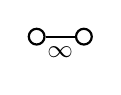
\begin{tikzpicture}[scale=\cgscale, auto, swap]
    % First we draw the vertices
    \foreach \pos/\name in {{(0,0)/a}, {(1,0)/b}}
        \node[vertex] (\name) at \pos {}; %{$\name$};
    % Connect vertices with edges and draw weights
    \foreach \source/ \dest /\weight in {a/b/\infty}
        \path[edge] (\source) -- node[weight] {$\weight$} (\dest);
\end{tikzpicture}}

\newcommand{\tildeAn}{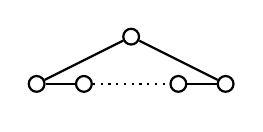
\begin{tikzpicture}[scale=\cgscale, auto, swap]
    % First we draw the vertices
    \foreach \pos/\name in {{(0,0)/a}, {(1,0)/b}, {(2,1)/c}, {(3,0)/d}, {(4,0)/e}}
        \node[vertex] (\name) at \pos {}; %{$\name$};
    % Connect vertices with edges and draw weights
    \foreach \source/ \dest /\weight in {a/b/,d/e/,a/c/,c/e/}
        \path[edge] (\source) -- node[weight] {$\weight$} (\dest);

    \path[edge, dotted] (b) -- node[weight] {} (d);
\end{tikzpicture}}

\newcommand{\tildeBCtwo}{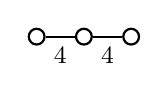
\begin{tikzpicture}[scale=\cgscale, auto, swap]
    % First we draw the vertices
    \foreach \pos/\name in {{(0,0)/a}, {(1,0)/b}, {(2,0)/c}}
        \node[vertex] (\name) at \pos {}; %{$\name$};
    % Connect vertices with edges and draw weights
    \foreach \source/ \dest /\weight in {a/b/4,b/c/4}
        \path[edge] (\source) -- node[weight] {$\weight$} (\dest);
\end{tikzpicture}}

\newcommand{\tildeBn}{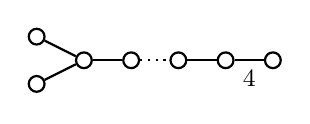
\begin{tikzpicture}[scale=\cgscale, auto, swap]
    % First we draw the vertices
    \foreach \pos/\name in {{(0,-0.5)/a}, {(0,0.5)/b}, {(1,0)/c}, {(2,0)/d}, {(3,0)/e}, {(4,0)/f}, {(5,0)/g}}
        \node[vertex] (\name) at \pos {}; %{$\name$};
    % Connect vertices with edges and draw weights
    \foreach \source/ \dest /\weight in {a/c/,b/c/,c/d/,e/f/,f/g/4}
        \path[edge] (\source) -- node[weight] {$\weight$} (\dest);

    \path[edge, dotted] (d) -- node[weight] {} (e);
\end{tikzpicture}}

\newcommand{\tildeCn}{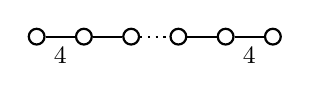
\begin{tikzpicture}[scale=\cgscale, auto, swap]
    % First we draw the vertices
    \foreach \pos/\name in {{(0,0)/a}, {(1,0)/c}, {(2,0)/d}, {(3,0)/e}, {(4,0)/f}, {(5,0)/g}}
        \node[vertex] (\name) at \pos {}; %{$\name$};
    % Connect vertices with edges and draw weights
    \foreach \source/ \dest /\weight in {a/c/4,c/d/,e/f/,f/g/4}
        \path[edge] (\source) -- node[weight] {$\weight$} (\dest);

    \path[edge, dotted] (d) -- node[weight] {} (e);
\end{tikzpicture}}

\newcommand{\tildeDn}{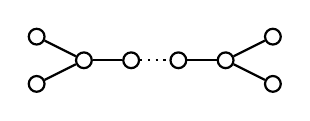
\begin{tikzpicture}[scale=\cgscale, auto, swap]
    % First we draw the vertices
    \foreach \pos/\name in {{(0,-0.5)/a}, {(0,0.5)/b}, {(1,0)/c}, {(2,0)/d}, {(3,0)/e}, {(4,0)/f}, {(5,-0.5)/g}, {(5,0.5)/h}}
        \node[vertex] (\name) at \pos {}; %{$\name$};
    % Connect vertices with edges and draw weights
    \foreach \source/ \dest /\weight in {a/c/,b/c/,c/d/,e/f/,f/g/,f/h/}
        \path[edge] (\source) -- node[weight] {$\weight$} (\dest);

    \path[edge, dotted] (d) -- node[weight] {} (e);
\end{tikzpicture}}

\newcommand{\tildeEsix}{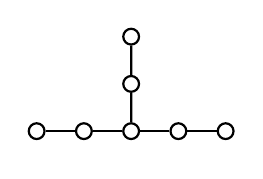
\begin{tikzpicture}[scale=\cgscale, auto, swap]
    % First we draw the vertices
    \foreach \pos/\name in {{(0,0)/a}, {(1,0)/b}, {(2,0)/c}, {(3,0)/d}, {(4,0)/e}, {(2,1)/f}, {(2,2)/g}}
        \node[vertex] (\name) at \pos {}; %{$\name$};
    % Connect vertices with edges and draw weights
    \foreach \source/ \dest /\weight in {a/b/,b/c/,c/d/,d/e/,c/f/,f/g/}
        \path[edge] (\source) -- node[weight] {$\weight$} (\dest);
\end{tikzpicture}}

\newcommand{\tildeEseven}{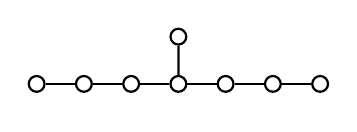
\begin{tikzpicture}[scale=\cgscale, auto, swap]
    % First we draw the vertices
    \foreach \pos/\name in {{(-1,0)/h}, {(0,0)/a}, {(1,0)/b}, {(2,0)/c}, {(3,0)/d}, {(4,0)/e}, {(5,0)/f}, {(2,1)/g}}
        \node[vertex] (\name) at \pos {}; %{$\name$};
    % Connect vertices with edges and draw weights
    \foreach \source/ \dest /\weight in {a/b/,b/c/,c/d/,d/e/,e/f/,c/g/,a/h/}
        \path[edge] (\source) -- node[weight] {$\weight$} (\dest);
\end{tikzpicture}}

\newcommand{\tildeEeight}{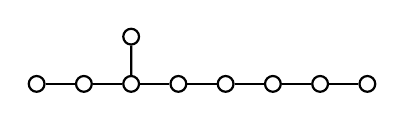
\begin{tikzpicture}[scale=\cgscale, auto, swap]
    % First we draw the vertices
    \foreach \pos/\name in {{(0,0)/a}, {(1,0)/b}, {(2,0)/c}, {(3,0)/d}, {(4,0)/e}, {(5,0)/f}, {(6,0)/g}, {(2,1)/h}, {(7,0)/i}}
        \node[vertex] (\name) at \pos {}; %{$\name$};
    % Connect vertices with edges and draw weights
    \foreach \source/ \dest /\weight in {a/b/,b/c/,c/d/,d/e/,e/f/,f/g/,c/h/,g/i/}
        \path[edge] (\source) -- node[weight] {$\weight$} (\dest);
\end{tikzpicture}}

\newcommand{\tildeFfour}{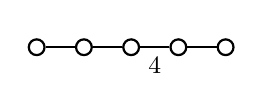
\begin{tikzpicture}[scale=\cgscale, auto, swap]
    % First we draw the vertices
    \foreach \pos/\name in {{(0,0)/a}, {(1,0)/b}, {(2,0)/c}, {(3,0)/d}, {(-1,0)/e}}
        \node[vertex] (\name) at \pos {}; %{$\name$};
    % Connect vertices with edges and draw weights
    \foreach \source/ \dest /\weight in {a/b/,b/c/4,c/d/,a/e/}
        \path[edge] (\source) -- node[weight] {$\weight$} (\dest);
\end{tikzpicture}}

\newcommand{\tildeGtwo}{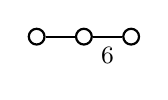
\begin{tikzpicture}[scale=\cgscale, auto, swap]
    % First we draw the vertices
    \foreach \pos/\name in {{(0,0)/a}, {(1,0)/b}, {(2,0)/c}}
        \node[vertex] (\name) at \pos {}; %{$\name$};
    % Connect vertices with edges and draw weights
    \foreach \source/ \dest /\weight in {a/b/,b/c/6}
        \path[edge] (\source) -- node[weight] {$\weight$} (\dest);
\end{tikzpicture}}

\newcommand{\Zfour}{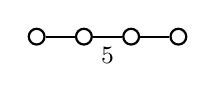
\begin{tikzpicture}[scale=\cgscale, auto, swap]
    % First we draw the vertices
    \foreach \pos/\name in {{(-1,0)/d}, {(0,0)/a}, {(1,0)/b}, {(2,0)/c}}
        \node[vertex] (\name) at \pos {}; %{$\name$};
    % Connect vertices with edges and draw weights
    \foreach \source/ \dest /\weight in {a/b/5,b/c/,d/a/}
        \path[edge] (\source) -- node[weight] {$\weight$} (\dest);
\end{tikzpicture}}

\newcommand{\Zfive}{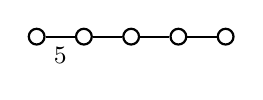
\begin{tikzpicture}[scale=\cgscale, auto, swap]
    % First we draw the vertices
    \foreach \pos/\name in {{(0,0)/a}, {(1,0)/b}, {(2,0)/c}, {(3,0)/d}, {(4,0)/e}}
        \node[vertex] (\name) at \pos {}; %{$\name$};
    % Connect vertices with edges and draw weights
    \foreach \source/ \dest /\weight in {a/b/5,b/c/,c/d/,d/e/}
        \path[edge] (\source) -- node[weight] {$\weight$} (\dest);
\end{tikzpicture}}